\documentclass[conference]{ieeetran}
\usepackage{authblk}
\usepackage{graphicx}
\graphicspath{ {./images/} }
%\usepackage{babel}
\usepackage{amsmath, amsfonts}

\usepackage[nottoc]{tocbibind}
\usepackage[european resistors, straightvoltages]{circuitikz}

\author[1]{Jay Piamjariyakul}
%\author[2]{Felix Kong}
\affil[1]{Undergraduate, Department of Electrical \& Electronic Engineering, University of Bristol}
%\affil[2]{Department of Mechanical Engineering, University of Bristol}
\title{Hot \& Motored: Generating Electricity with Footsteps}

\renewcommand\IEEEkeywordsname{Keywords}
\newcommand{\figref}[1]{\figurename~\ref{#1}}
\newcommand{\compref}[1]{Comp.~\ref{#1}}
\newcommand{\stepref}[1]{Step~\ref{#1}}

\begin{document}

\maketitle
\begin{abstract}
This document examines the plausibility \& efficiency of generating power via footsteps, which could be used on pavements to generate electricity used for various purposes, depending on the user's preferences.
\\
Excuse the pun.
\end{abstract}

% \begin{IEEEkeywords}
%     Component (comp.)
% \end{IEEEkeywords}
 
% \section{Preamble}
% The application of utilising footsteps to generate electricity adapts the mechanisms of a dynamo (which generates electricity from mechanical torque input) and that of a pressure plate (akin to those used in vintage spinning-top toys). Its applications, theoretically, could be used to alleviate lack of electricity in remote regions (given a large amount of foot-based commuting) or help local businesses collect data in regards to visitors/browsers \& determine their best course of business action.

\section{Mechanism Proposal}
The proposed mechanism to generate electricity is comprised of multiple components, and such operate in unison to provide the output voltage at the output stage.

\subsection{Components Analysis}
The mechanism itself involves a button/plate that, when pressed, would push a spiral down an entry point, compressing a spring. When such button/plate (thus, the spring) is released, the spiral is released to its initial position, in turn spinning the flywheel disc/gear that such spiral is fixed to, causing such to move in a rotational manner.

\begin{figure}[ht]
    \centering
    \caption{Diagram of proposed mechanism to generate electricity from footsteps}
    \label{fig:mech_wlabel}
    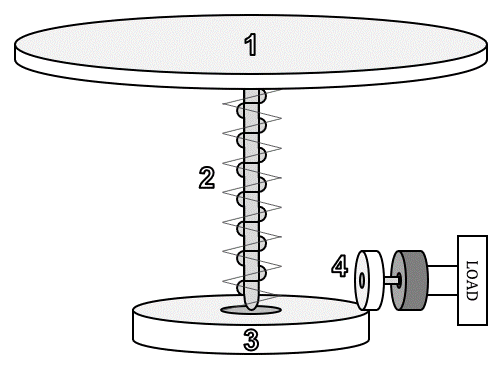
\includegraphics[width=\linewidth]{mech_wlabel.png}
\end{figure}

Such mechanism is shown in \figref{fig:mech_wlabel} and is comprised of the following components (refer to labels on \figref{fig:mech_wlabel}):
\begin{enumerate}
    \item\label{item:comp:plate} Plate which individual steps onto - such is supported by a compression spring
    \item\label{item:comp:spiral} Spiral rod which inserts into \compref{item:comp:flywheel}'s axle - such is attached to \compref{item:comp:plate}
    \item\label{item:comp:flywheel} Flywheel which \compref{item:comp:spiral} inserts into via an opening fitting the size of the spiral's rectangular body
    \item\label{item:comp:motor} Motor with additional gears connected to \compref{item:comp:flywheel}, where such is repurposed as a generator; such gears may include transmission stages
\end{enumerate}

\subsection{Operations of Mechanism}
The mechanism is intended to operate per the following procedures (refer to labels on \figref{fig:mech_wlabel}):
\begin{enumerate}
    \item\label{item:op:stepdn} One steps onto \compref{item:comp:plate}, pushing \compref{item:comp:spiral} downwards \& compressing the support spring
    \item\label{item:op:spiraldn} \compref{item:comp:spiral} moving downwards passes through slot in \compref{item:comp:flywheel}
    \item\label{item:op:stepup} One steps away from \compref{item:comp:plate}, resulting in the spring being released; such results in \compref{item:comp:spiral} moving upwards to its original position
    \item\label{item:op:spin} \compref{item:comp:spiral} moving upwards now results in \compref{item:comp:flywheel} rotating, causing \compref{item:comp:motor}'s axle to also be rotated (due to the bevel gear connection)
    \item\label{item:op:induce} The rotation of \compref{item:comp:motor}'s axle results in EMF being generated at its output
\end{enumerate}

One can surmise that power from \textbf{linear motion} (due to Steps \ref{item:op:stepdn} and \ref{item:op:spiraldn}) is converted to that of \textbf{rotary motion} (given by Step \ref{item:op:spin}), and later converted via \textbf{induction} (per Step \ref{item:op:induce}).

% ------------------------------
% ------------------------------

\section{Theory}
% Insert brief intro of section
This section concerns the generator's output characteristics \& how such is linked to the mechanical stage prior. Such refers to \cite{industrial2} in regards to theory \& formula behind such operations.

%Generating electricity from footsteps adapts the fundamental theorems of mechatronics, prominent those involving electromagnetic induction. See \cite{industrial2} for reference.

%\subsection{Electromagnetic Induction}
% One recalls Faraday's \textbf{Law of Electromagnetic Induction} (and Lenz' Law)
% \begin{equation}
%     % Use \varepsilon for curly epsilon
%     \epsilon = -\frac{d\psi}{dt} \equiv -N\frac{d\phi}{dt} = -N\frac{dBA}{dt}
%     \label{eq:faraday}
% \end{equation}
% where such terms are defined per following:
% \begin{itemize}
%     \item \(\epsilon\): \textbf{EMF} generated within coil (V)
%     \item \(\psi\): magnetic \textbf{flux linkage} (Wb Turns)
%     \item \(\phi\): magnetic \textbf{flux} (Wb)
%     \item \(N\): amount of wire turns within a coil (Turns)
%     \item \(B\): magnetic flux density (T)
%     \item \(A\): area of coil (m\(^2\))
% \end{itemize}

% \begin{displaymath}
%     \epsilon = -NA\frac{dB}{dt}
% \end{displaymath}

\subsection{Generator Output Characteristics}
The generator's output mechanism can be modelled as an equivalent circuit per \figref{circuit:generator}, where the following terms are defined:
\begin{itemize}
    \item $\omega$/$T$: Angular speed \& torque of generator's input axle, dictated by its transmission gear \& stages
    \item $E$: Output EMF of generator
    \item $\mathcal{R}_a$: Generator reluctance
    \item $I_a$/$V_a$: Current \& voltage at load output of generator
\end{itemize}

\begin{figure}[ht]
    \centering
    \label{circuit:generator}
    \caption{Equivalent circuit of generator and its output}
    \begin{circuitikz}
        \draw (0, 0) to[Telmech=G, n=generator] (0, 2) to[short, -*] (1, 2);
        \draw (1, 2) to[R=\text{\(\mathcal{R}_a\)}, i=\(I_a\), -o] (4,2);
        \draw (1, 0) to [open, v>=$E$] (1, 2);
        \draw (0, 0) to[short, -*] (1, 0) to[short, -o] (4, 0);
        \draw (4, 0) to [open, v>=$V_{a}$] (4, 2);
        \draw [thick, ->>] (-1.5, 1) -- (generator.left) node[
            midway,above]{$\omega$} node[
                midway,below]{$T$};
    \end{circuitikz}
\end{figure}

Such is governed by the equations given by \eqref{eq:dcmotor}, where $k_e$ is the \textbf{electromagnetic constant} of the motor/generator.
\begin{equation}
    \label{eq:dcmotor}
    \begin{aligned}
        T &= k_e I_a\\
        E &= k_e \omega
    \end{aligned}
\end{equation}

Given \figref{circuit:generator} one can surmise the following information given by \eqref{eq:circuit} and \eqref{eq:dcmotor}.
\begin{equation}
    \label{eq:circuit}
    \begin{aligned}
        V_a &= E - I_aR_a\\
        &= k_e\omega - \left(\frac{T}{k_e}\right)R_a
    \end{aligned}
\end{equation}

\subsection{Mechanical Input Characteristics}
% Calculate general omega/tau from spiral rod!!

\medskip
\bibliographystyle{IEEEtran}
\bibliography{references}

\end{document}